%Die Angabe des schlauen Spruchs auf diesem Wege funtioniert nur,
%wenn keine Änderung des Kapitels mittels den in preambel/chapterheads.tex
%vorgeschlagenen Möglichkeiten durchgeführt wurde.
%\setchapterpreamble[u]{%
%\dictum[Albert Einstein]{Probleme kann man niemals mit derselben Denkweise lösen, durch die sie entstanden sind.}
%}
\chapter{Realisierung}
\label{chap:impl}
Neben der mathematischen Ausarbeitung (siehe \autoref{chap:maths}) beschäftigt sich diese Arbeit auch mit der eigentlichen Implementierung des erarbeiteten Verfahrens. In diesem Kapitel werden die Anforderungen an die Software sowie das Vorgehen bei der Wahl der Programmiersprache beschrieben. Anschließend werden die Installation und Bedienung kurz erklärt. Es folgt eine Auflistung der externen Bibliotheken die zum Einsatz kamen und eine Beschreibung der Architektur der Software.

%------------------------------------------------------------------------------------------------------------------------------------
\section{Anforderungen}
Die Anforderungen an die Realisierung der Arbeit lassen sich zum einen aus der Aufgabenbeschreibung der Bachelor-Arbeit entnehmen und sind zum anderen während der Bearbeitung des theoretischen Ansatzes entstanden. Diese lassen sich in funktionale und nichtfunktionale Anforderungen gliedern  \cite[S. 369f]{ludewig}.
\subsection{Funktionale Anforderungen}
\label{fa}
\begin{description}
\item[Evaluation der Daten:] Die entstehenden Daten sollen evaluiert und grafisch dargestellt werden. Dazu muss die Software in der Lage sein folgende Aufgaben zu übernehmen: 
    \begin{itemize}
        \item Anpassung der Parameter für die Berechnung des \gls{HDR}-Bildes
        \item Darstellung der Antwortkurve $\b g$ als grafischen Plot
        \item Anzeigen des \gls{HDR}-Bildes mit verschiedenen \gls{Tone-Mapping}-Operatoren
        \item Änderung der Parameter der \gls{Tone-Mapping}-Operatoren
    \end{itemize}
    
\item[Mathematische Korrektheit:] Bei dieser Implementierung handelt es sich um eine interdisziplinäre Aufgabe. Die Berechnung des \gls{HDR}-Bildes muss mathematisch korrekt ablaufen und soll der mathematischen Ausarbeitung (siehe \autoref{chap:maths}) entsprechen. Die Formulierung des Optimierungsproblems in effektiven Programmcode stellt deswegen eine besondere Herausforderung dar. Um die mathematische Korrektheit zu gewährleisten, sind umfassende Tests der mathematischen Klassen und Hilfsmethoden notwendig.

\item[Reproduzierbarkeit:] Die Berechnungen des Programms sollen reproduzierbar sein. Dadurch ist eine Evaluation der Daten unter verschiedenen Eingaben möglich.

\end{description}


\subsection{Nichtfunktionale Anforderungen}
\label{nfa}
\begin{description}
    \item[Portierbarkeit:] Die Implementierung der Software soll auf verschiedene Systeme portierbar sein. Dazu gehören \texttt{Windows}, \texttt{MacOS} und \texttt{Linux}-Derivate. Die eingesetzte Programmiersprache soll dies ohne weitere Probleme ermöglichen.
    
    \item[Performanz:] An die Performanz der Implementierung wurden keine besonderen Anforderungen gestellt. Die Umsetzbarkeit und die Ausgabe des Programms stehen im Vordergrund. Aus diesem Grund wurde von einer Laufzeitanalyse des Programmes abgesehen.
    
    \item[Software-Qualität:] Da diese Arbeit eine Bachelor-Arbeit der Fachrichtung \textit{Softwaretechnik} ist, bestehen Anforderungen an die Qualität des Quellcodes. Diese beinhaltet die folgenden Aspekte.
    \begin{itemize}
        \item Automatisierte Modul-Tests (Zielwert: 90\% Anweisungsüberdeckung für das Paket \texttt{Maths}, 80\% Anweisungsüberdeckung für das Paket \texttt{Solve}, 90\% Anweisungsüberdeckung für das Paket \texttt{Model}, für die Pakete \texttt{View} und \texttt{Ctrl} besteht keine Anforderung)
        \item \gls{OOP}
        \item Die Module und \texttt{public} Funktionen werden gemäß dem offiziellem Javadoc Style Guide\footnote{\url{http://www.oracle.com/technetwork/java/javase/documentation/index-137868.html}} kommentiert
        \item Erstellung einer Software-Dokumentation (z.B. \texttt{JavaDoc})
        \item Gliederung des Programms in Pakete
    \end{itemize}
    \item[\Gls{GUI}:] Die \gls{GUI} soll es dem Benutzer erlauben, dem Algorithmus Bildserien und die benötigten Parameter für die Generierung eines \gls{HDR}-Bildes einzugeben. Dazu gehören folgende Aspekte:
    \begin{itemize}
        \item Eingabe der Bildserie
        \item Eingabe der Parameter für die Bildgenerierung
        \item Eine Einweisung soll nicht erforderlich sein
        \item Validierung der Eingaben des Benutzers
    \end{itemize}

    Darüber hinaus soll der Benutzer über den Stand der Berechnung informiert werden und Zwischenergebnisse sehen können. 
    
    \item[Robustheit:] Bei Fehlern oder Problemen in der Software soll eine adäquate Fehlerbeschreibung geliefert werden. Das betrifft sowohl fehlerhafte Eingaben, als auch Programmfehler während der Berechnung.
\end{description}




%------------------------------------------------------------------------------------------------------------------------------------
\section{Wahl der Programmiersprache}
\label{sec:language}
Für die Implementierung des Programms wurde eine Analyse verschiedener Programmiersprachen durchgeführt. Eine Übersicht der untersuchten Sprachen ist in \autoref{tab:languages} zu finden. Der Vergleich zeigt, dass \texttt{Go} und \texttt{C} aufgrund der fehlenden Möglichkeit zur \gls{OOP} ausscheiden. Die verbleibenden vier Sprachen \texttt{Java}, \texttt{C++}, \texttt{C\#}  und \texttt{Free Pascal} unterscheiden sich dann nur noch kaum. Lediglich die Erstellung einer \gls{GUI} und die integration von automatisierten Tests werden von den beiden zuletzt genannten Sprachen nur über zusätzliche Bibliotheken unterstützt. \texttt{Java} schließt nur in Punkto nativem Systemzugriff und damit der Performance schlechter ab, als die anderen Sprachen im Test. Da jedoch an die Performanz der Software (siehe \autoref{nfa}) keine besonderen Anforderungen gestellt waren, ist dieser Punkt zu vernachlässigen. 

\begin{table}[H]
  \begin{center}
    \begin{tabular}{l|c|c|c|c|c|c}
	\toprule
      Sprache 
          & \texttt{Java} 
          & \texttt{C} 
          & \texttt{C\#} 
          & \texttt{C++} 
          & \texttt{Object Pascal\footnote{Implementierung: \texttt{Free Pascal}}} 
          & \texttt{Go}\\ 
      \midrule
      
      Portierbarkeit 
          & \checkmark 
          & \checkmark 
          & (\checkmark)\footnote{Plattformunabhängige Realisierung mit \texttt{Mono} (siehe \url{http://www.mono-project.com})} 
          & \checkmark 
          & \checkmark
          &\checkmark \\
      
      \gls{GUI} 
          & \checkmark 
          & (\checkmark)\footnote{z.B. \texttt{GTK+} (\url{http://www.gtk.org})} 
          & \checkmark 
          & (\checkmark)\footnote{z.B. \texttt{Qt} (\url{http://qt-project.org})}
          & \checkmark\footnote{z.B. Integration in der IDE \texttt{Lazarus} (\url{http://www.lazarus.freepascal.org})} 
          & (\checkmark)\footnote{z.B. \texttt{go-gtk} (\url{http://mattn.github.io/go-gtk/})}\\
      
      \gls{OOP}
          & \checkmark 
          & $\times$  
          & \checkmark 
          & \checkmark 
          & \checkmark 
          & $\times$\\
      
      Automatisierte Tests 
          & \checkmark 
          & (\checkmark)\footnote{z.B. \texttt{Check} (\url{http://check.sourceforge.net})} 
          & \checkmark 
          & (\checkmark)\footnote{z.B. \texttt{CppUnit} (\url{http://cppunit.sourceforge.net})}
          & (\checkmark)\footnote{z.B. \texttt{FPCUnit} (\url{http://wiki.freepascal.org/fpcunit})}
          & \checkmark \\
      
      Nativer Systemzugriff
          & $\times$\footnote{Virtuelle Maschine (\gls{JRE})} 
          & \checkmark 
          & \checkmark 
          & \checkmark
          & \checkmark
          & \checkmark
          \\
	\bottomrule
    \end{tabular}
    \caption{Vergleich der Programmiersprachen mit den Anforderungen. (\checkmark: \textit{out of the box}, (\checkmark): zusätzliche Bibliotheke oder Erweiterung benötigt, $\times$ keine Unterstützung)}
    \label{tab:languages}
  \end{center}
\end{table}


Aufgrund meiner in universitären Projekte erlangten Vorkenntnissen in \texttt{Java} und des besseren Abschneidens im Vergleich mit den anderen hier genannten Sprachen, wird die Software in \texttt{Java} realisiert.


\section{Programmvorstellung und Benutzeroberfläche}

Für die Realisierung der \gls{GUI} und der grafische Evaluation der Ergebnisse wurde in der vorliegende Arbeit eine \texttt{Swing}-Oberfläche (siehe \autoref{fig:tool}) implementiert, die sowohl die Eingabe der Parameter und Daten als auch die Ausgabe der verschiedenen Diagramme und Bilder ermöglichen soll. In der nachfolgenden Beschreibung sind die umgesetzten Anforderungen zu erkennen.

Über den Button \enquote{Bilder wählen} können die Eingabebilder gewählt werden. Im dafür entwickelten Datei-Fenster steht dem Benutzer eine Vorschau der Bilder zur Verfügung. Aus Gründen der Robustheit (siehe \autoref{nfa}) können nur Bilddateien ausgewählt werden.  Eine Registrierung der Bilder wird nicht unterstützt. Dies bedeutet, dass die Bilder vorab von Hand oder mit einem Algorithmus registriert werden müssen. Der Nutzer erhält diesbezüglich einen Hinweis bei der Auswahl der Bilder.

In der Tabelle im unteren Bereich des Fensters werden die Bilder mit ihren Belichtungszeiten aufgeführt. Falls die Bibliothek \texttt{metadate-extractor} die Belichtungszeiten nicht auslesen konnte müssen diese händisch eingegeben werden. Auch hierzu erhält der Benutzer ggf. einen optischen Hinweis.

Die Verwendung der Komponente \texttt{NumericTextField} (siehe \autoref{externals}) bei der Eingabe der Parameter stellt sicher, dass der Benutzer nur sinnvolle Daten angibt. Bei Falscheingaben ertönt ein akustisches Warnsignal. Die \enquote{Start} Schaltfläche wird bei fehlenden oder fehlerhaften Angaben deaktiviert. Die Eingabemöglichkeiten werden deaktiviert sobald der Berechnungsprozess gestartet wird. Dies verhindert ungültige Benutzerinteraktionen. Das Anwendungsfenster verfügt zudem über eine Fortschrittsanzeige im unteren Bereich. Detaillierte Informationen über den Fortgang der Berechnung können im \texttt{LOG}-Reiter der Anwendung eingesehen werden.

\subsection{Installation}

Die Anwendung kann unter \url{https://github.com/sebastianzillessen/hdr-generator} heruntergeladen werden. Dazu wird ein installiertes \gls{JRE} der Version 6 oder höher benötigt (siehe \url{http://www.java.com/de/download/}). Im Unterordner \texttt{bin} befindet sich eine ausführbare Version des Programms als \texttt{.jar} Datei. 

\begin{figure}
  \begin{center}
    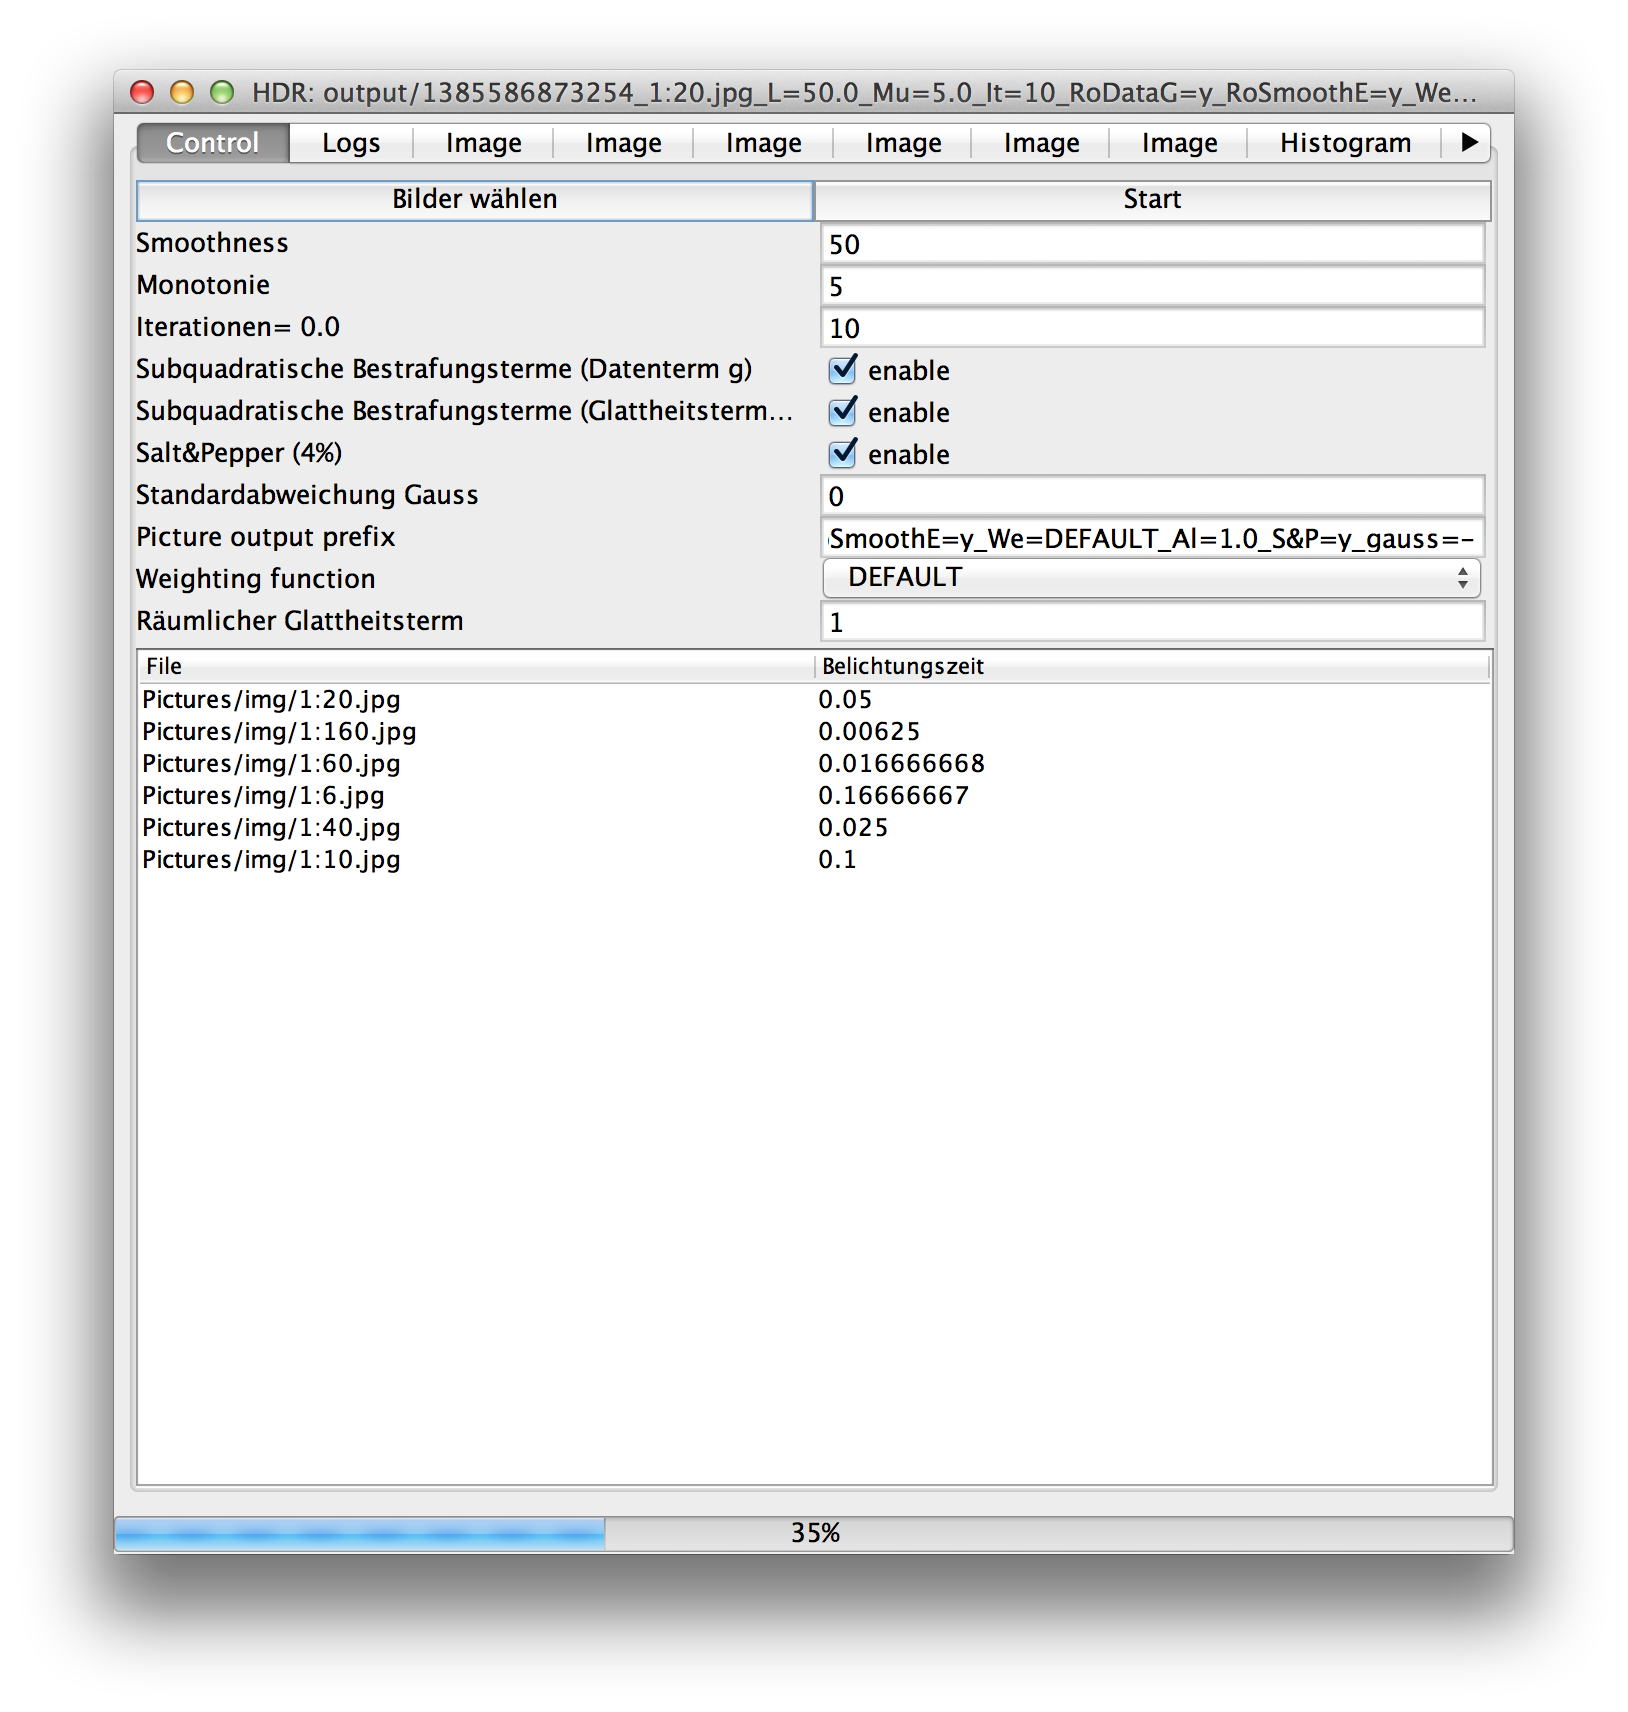
\includegraphics[width=0.5\textwidth]{Tool}
    \caption{Die Benutzereingabe für die Erzeugung der HDR-Bilder ist absichtlich schlicht und einfach gehalten.}
    \label{fig:tool}
  \end{center}
\end{figure}


\subsection{Erste Schritte}
Nach dem Öffnen der Anwendung erscheint das Hauptfenster (siehe \autoref{fig:tool}). Folgende Schritte sind notwendig um ein \gls{HDR}-Bild zu erzeugen:

\begin{enumerate}
    \item Wahl der Belichtungsserie über die Schaltfläche \enquote{Bilder wählen}.
    \item Eingabe der Belichtungszeiten in der Tabelle (falls notwendig).
    \item Veränderung der Parameter für die Bilderzeugung (falls gewünscht). Dazu gehören:
    \begin{itemize}
        \item Gewichtung der Glattheitsforderung $\lambda$ von $\b g$
        \item Monotonie-Forderung durch die Eingabe des Gewichtes $\mu$
        \item Anzahl der Haupt- und Inneniterationen (siehe \autoref{alg:alternierend:extended})
        \item Aktivierung des Räumlichen Glattheitsterms 
        \item Aktivierung der subquadratischen Bestrafungsterme für $\b g$ und $\b E$, sowie für den räumlichen Glattheitsterm
        \item Bildstörungen (\gls{SaltAndPepperNoise} oder additives Gauss-Rauschen) auf den Eingabebildern (zu Testzwecken)
        \item Änderung des Prefix für den Export von Bildern
    \end{itemize}

    \item Bestätigung der Generierung mittels der Schaltfläche \enquote{Start}.
\end{enumerate}

Dadurch wird das \gls{HDR}-Bild erzeugt. Der Fortschritt wird im unteren Bereich dargestellt. Die Ausgabe (auch der Zwischenresultate) erfolgt über die verschiedenen Reiter des Fensters. Bei der Darstellung des \gls{HDR}-Bilds mit den verschiedenen \gls{Tone-Mapping}-Operatoren können die Parameter in der Oberfläche verändert werden (siehe \autoref{fig:app:tone}). Der Export der generierten Bilder und Kurven erfolgt über die Schaltfläche \enquote{Speichern}.

\begin{figure}
  \begin{center}
    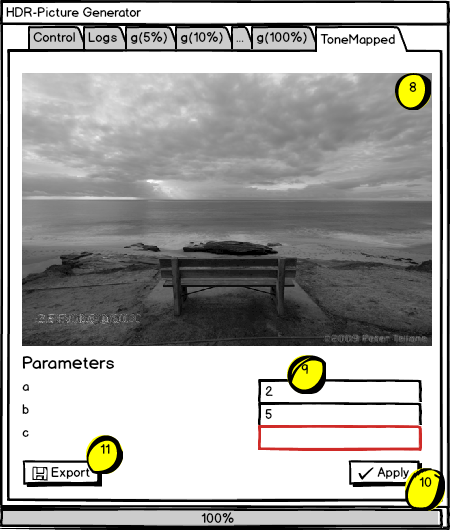
\includegraphics[width=0.5\textwidth]{tonemapped}
    \caption{Vorschau des Tone-Mapped Resultats mit der Möglichkeit der Veränderung der Variablen für diesen Tone-Mapper (globaler \gls{Tone-Mapping}-Operator von Reinhard).}
    \label{fig:app:tone}
  \end{center}
\end{figure}




%------------------------------------------------------------------------------------------------------------------------------------





%------------------------------------------------------------------------------------------------------------------------------------

\section{Architektur}
\label{sec:architektur}
Bei der Architektur der Software wurde eine \gls{MVC} Struktur eingehalten. Dieses Muster beschreibt eine klare Trennung zwischen Datendarstellung, -verarbeitung und -repräsentation. Diese Teilung in drei Schichten sorgt dafür, dass die einzelnen Komponenten gut getestet werden können und beliebig austauschbar sind. Dadurch besteht ein hoher Grad an Erweiterbarkeit, da die Kopplung zwischen den Modulen gering ist \cite[S.~413]{ludewig}.

In allen Klassen wurde grundsätzlich das Prinzip des \textit{information hiding} angewandt, wodurch eine verbesserte Erweiterbarkeit durch klare Schnittstellen gegeben ist.

\begin{ieee}{information hiding}
A software development technique in which each module's interfaces reveal a s little a s possible about the module's inner workings and other modules are prevented from using information about the module that is not in the module's interface specification.
\end{ieee}

\subsection{Paketdiagramm}
Die Anwendung lässt sich in fünf verschiedene Pakete trennen (siehe \autoref{fig:arch:components}). Die Zuordnung zu den drei Schichten ist in den (\textit{\texttt{Klammern}}) angegeben.
\begin{description}



\item{\texttt{View} (\textit{\texttt{View}}):} Das Paket \texttt{View} behandelt die gesamte Darstellung der Anwendung und die grafische Auswertung der berechneten Bilder. Es enthält \gls{Tone-Mapping}-Operatoren und behandelt die Benutzereingabe.

\item{\texttt{Ctrl} (\textit{\texttt{Controller}}):} Dieses Paket dient zur Steuerung der Anwendung. Es werden die Eingaben verarbeitet, an die Algorithmen übergeben und an die \texttt{View} zurückgegeben.

\item{\texttt{Model} (\textit{\texttt{Model}}):} Das \texttt{Model} besteht in erster Linie aus den beiden Klassen \texttt{Image} und \texttt{HDRResult} und ist damit ein Datentypmodul \cite[S. 412]{ludewig}. Erstere wird als Repräsentation eines Bildes verwendet und speichert Grauwerte, Belichtungszeiten und weitere bildrelevante Informationen. Letztere dient als Kommunikationspaket zwischen dem eigentlichen \texttt{Solver} und der restlichen Anwendung und enthält die fertig berechnete Antwortkurve und die \gls{Radiance Map}. 

\item{\texttt{Solver} (\textit{\texttt{Model}}):} Der \texttt{Solver} ist der eigentliche Kern des Programms. In diesem Paket wird die Bestimmung der Antwortkurve $\b g$ sowie die Berechnung der \gls{Radiance Map} behandelt. Hier fließen die mathematischen Erkenntnisse aus \autoref{chap:maths} ein. 

\item{\texttt{Maths} (\textit{\texttt{Model}}):} Die \texttt{Maths}-Komponente ist ein Funktionales Modul \cite[S. 412]{ludewig}. Es enthält alle notwendigen mathematischen Berechnungen und Repräsentationen, wie z.B. \texttt{Matrix} und \texttt{Vector}.
\end{description}


Nachfolgend wird nun auf die einzelnen Pakete und Klassen näher eingegangen (siehe \autoref{fig:arch:view}). Die \texttt{View} besteht in erster Linie aus der Klasse \texttt{GuiFrame}. Diese ist das eigentliche Fenster des Programms und übernimmt die Schnittstelle zwischen Anwender und Programm. 

Darin enthalten sind auch die verschiedenen \texttt{ToneMappers}, die zur Darstellung der \gls{Radiance Map} verwendet werden ( Paket \texttt{Plots}).

\begin{figure}
  \begin{center}
    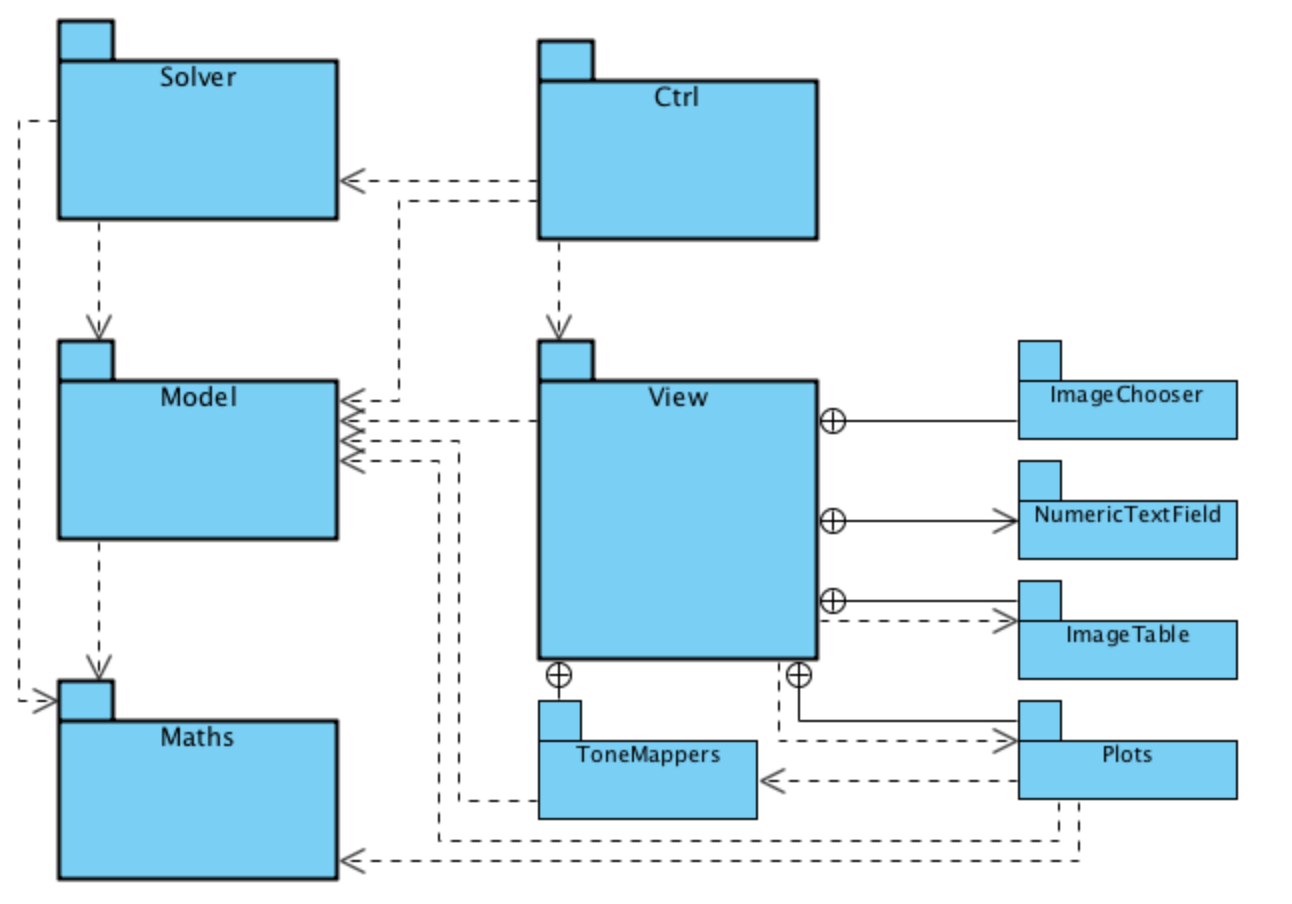
\includegraphics[width=0.6\textwidth]{architecture/components}
    \caption{Die Architektur der Software auf Paketebene. Die fünf Hauptpakete sind \texttt{Solver}, \texttt{View},\texttt{Ctrl}, \texttt{Model}, \texttt{Maths} (hier fett dargestellt).  Die übrigen fünf Pakete (\texttt{ToneMappers}, \texttt{ImageChooser}, \texttt{ImageTable}, \texttt{Plots} und \texttt{NumericTextField} sind im Paket \texttt{View} enthalten und werden hier für einen besseren Überblick ebenfalls dargestellt.}
    \label{fig:arch:components}
  \end{center}
\end{figure}


\begin{figure}
  \begin{center}
    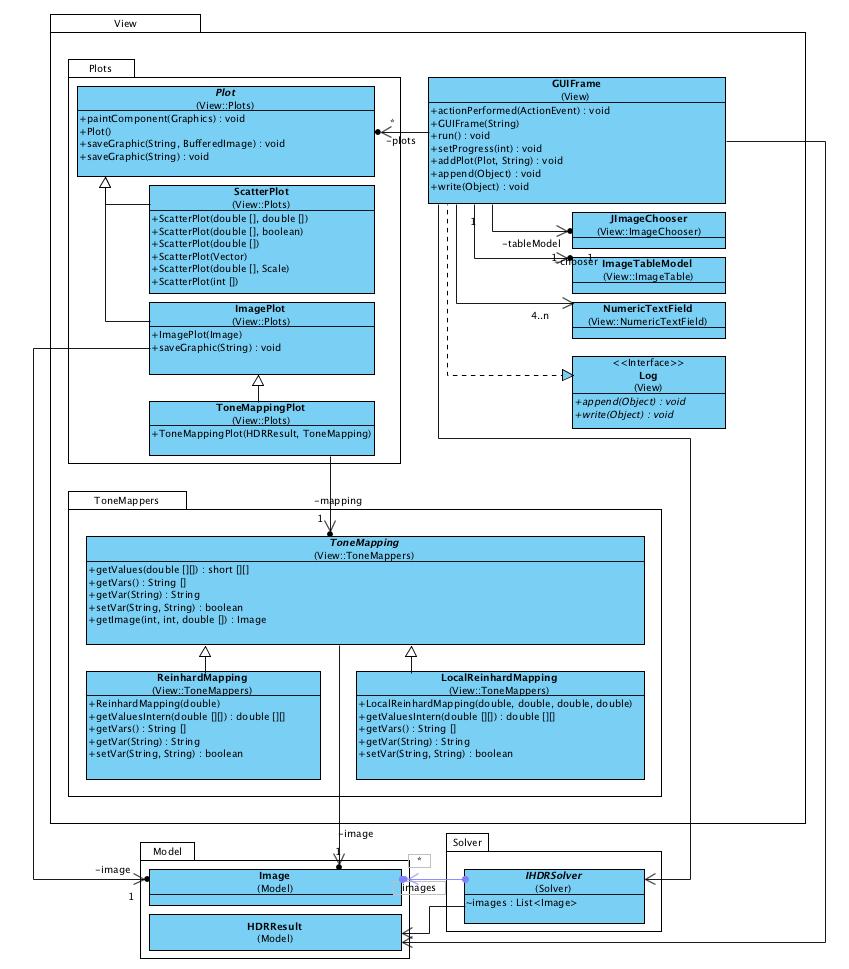
\includegraphics[width=0.8\textwidth]{architecture/view}
    \caption{Das \texttt{View}-Paket im Detail. Das Hauptfenster \texttt{GUIFrame} stellt die zentrale Klasse für die Darstellung dar und importiert dazu die verschiedenen Komponenten. Die \texttt{Plots} und die \texttt{ToneMappers} gehören ebenfalls zu diesem Paket.}
    \label{fig:arch:view}
  \end{center}
\end{figure}

Alle rein mathematischen Aufgaben (wie z.B. die LU-Zerlegung oder das SOR-Verfahren, siehe \autoref{sec:solvers}) sind im Paket \texttt{Maths} ausgelagert, da dieses Paket die gesamte mathematische Logik enthalten soll. So kann -- bei Bedarf -- auf eine andere Bibliothek für das Lösen der mathematischen Probleme (in aller erster Linie der Gleichungssysteme) gewechselt werden, ohne die Logik des erarbeiten Lösungsalgorithmus zu verändern. 

Die abstrakte Klasse \textit{\texttt{AbstractMatrix}} stellt die Basisfunktionalität im Umgang mit Matrizen zur Verfügung und kennt die beiden Implementierungen \texttt{BandMatrix} und \texttt{Matrix}. Erstere ist eine spezielle Repräsentation von dünnbesetzten Diagonalmatrizen mit beliebig vielen Bändern. Die hier häufig beschriebenen pentadiagonal Matrizen werden mit dieser Implementierung dargestellt. Der Vorteil dieser ist, dass auch große sehr dünn besetzte Matrizen abgespeichert werden können (in einem zweidimensionalen Array würden diese zu viel Speicherplatz verbrauchen). Die \texttt{Matrix} ist die zweite Implementierung der Matrizen und arbeitet intern mit einem zweidimensionalen Array.

Die Klasse \texttt{EquationSolver} (Paket \texttt{Maths}) übernimmt das Lösen eines \gls{LGS}. Das \gls{SOR}- und das LU-Verfahren werden unterstützt. Die beiden Hilfsklassen \texttt{Convolution} und \texttt{ArrayMaths} bieten weitere Berechnungsfunktionalitäten, die z.B. in den \gls{Tone-Mapping}-Verfahren verwendet werden. 
\begin{figure}
  \begin{center}
    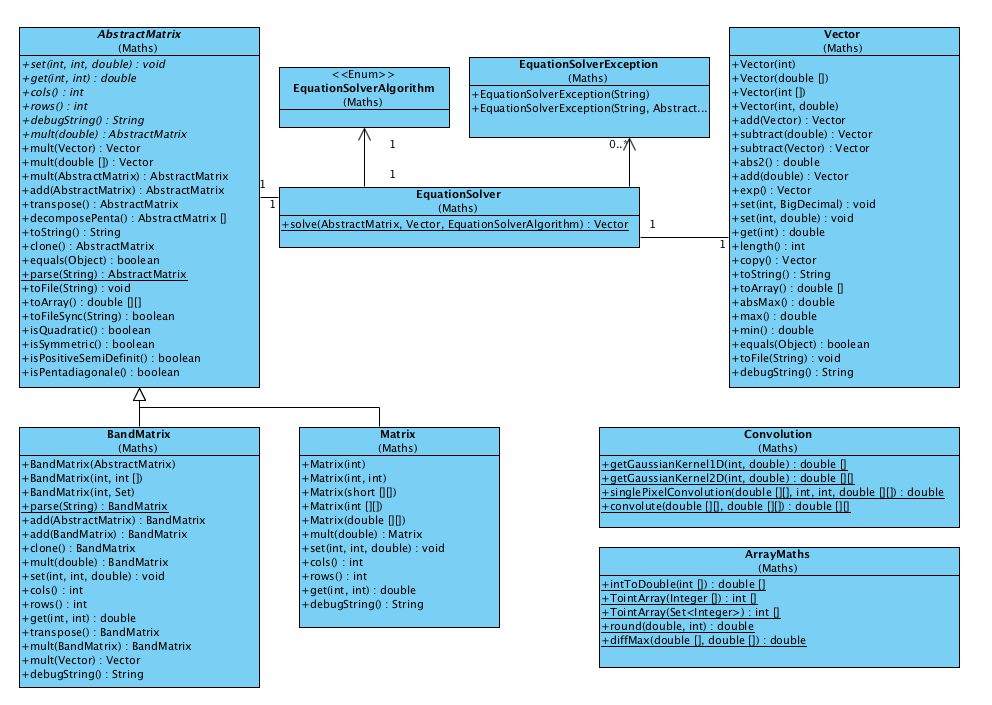
\includegraphics[width=0.9\textwidth]{architecture/maths}
    \caption{Überblick über das Paket \texttt{Maths}. Auf die Darstellung der Assoziationen zu den restlichen Klassen und Paketen wurde aus Gründen der Übersichtlichkeit verzichtet.}
    \label{fig:arch:matrix}
  \end{center}
\end{figure}

\subsection{Sequenzdiagramm}
Das Programm läuft sehr vielschichtig ab. Als grundsätzlicher Informationsfluss dient der Aufbau wie er in \autoref{fig:arch:sequence} beschrieben. Wichtig dabei ist, dass die grafische Benutzeroberfläche nicht von der Berechnungsdauer des Algorithmus blockiert wird, da so die Zwischenresultate des Algorithmus bereits analysiert werden können und der Prozess ggf. früher beendet werden kann um Parameter zu verändern. Deshalb bestehen besonders zwischen \texttt{Controller} und \texttt{GUIFrame} asynchrone Methodenaufrufe. Das Sequenzdiagramm ist nur beispielhaft zu verstehen. Es wurden einige Aufrufe und Zwischenschritte vereinfacht oder weggelassen.
\begin{figure}
  \begin{center}
    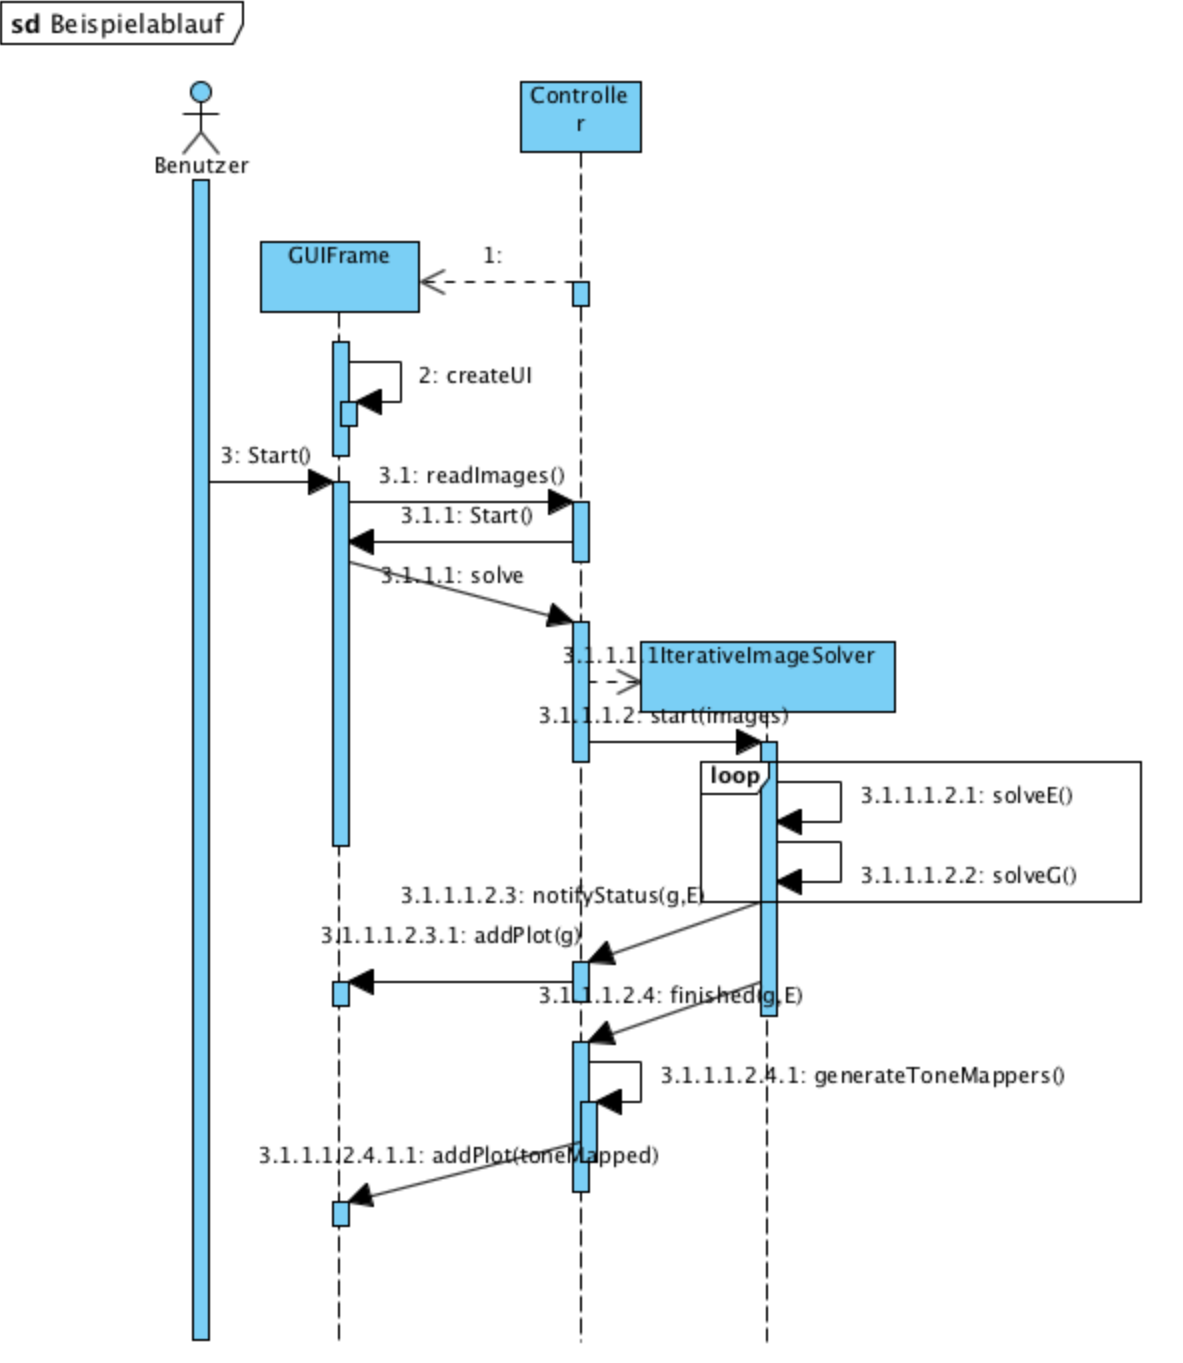
\includegraphics[width=\textwidth]{architecture/sequence_example}
    \caption{Der grundsätzliche Ablauf der Berechnung des HDR-Bildes und der Antwortkurve und der dabei beteiligten Komponenten sowie deren Interaktion. Zwischenschritte und tiefer verschachtelte Aufrufe werden nicht dargestellt. }
    \label{fig:arch:sequence}
  \end{center}
\end{figure}


%------------------------------------------------------------------------------------------------------------------------------------
\section{Externe Bibliotheken}
\label{externals}
Für die Implementierung wurden einige externen Komponenten verwendet. Diese werden hier kurz beschrieben.
\begin{description}
\item[\texttt{NumericTextField}\footnote{\url{http://www.java2s.com/Code/Java/Swing-JFC/NumericTextField.htm}}]
Für die Eingabe der einzelnen Parameter wird eine Implementierung eines numerischen Textfeldes verwendet. Dieses verhindert ungültige Eingaben und erleichtert das Auslesen der numerischen Parameter. Diese Komponente verwendet mehrere Klassen und wurde deshalb in den nachfolgenden Diagrammen zu einem Paket gebündelt.

\item[\texttt{metadata-extractor}\footnote{\url{https://code.google.com/p/metadata-extractor/}}]
Die Bibliothek \texttt{metadata-extractor} wird verwendet um automatisiert aus Bilddateien die Belichtungszeit der Bilder auszulesen. Mit dieser wird auch das von Adobe entwickelte \texttt{xmp-core}\footnote{\url{http://www.adobe.com/devnet/xmp.html}} mit geliefert. Zusammen ermöglichen es die Bibliotheken die Belichtungszeiten der Bilder auszulesen und darzustellen.

\item[\texttt{JImageChooser} \footnote{\url{http://docs.oracle.com/javase/tutorial/uiswing/examples/components/index.html\#FileChooserDemo2}}]
Der verwendete \texttt{JFileChooser} zur Selektion der Bilddateien ist inspiriert von dem vorhandenen Tutorial bei Oracle. Er ist in der Lage eine kleine Vorschau der Bilder anzuzeigen.
\end{description}

\section{Herausforderungen während der Programmierung}

\texttt{T.B.D, ggf. rauslassen}